\documentclass[12pt]{article}
\usepackage{amsmath}
\usepackage{amssymb} %mathbb
\usepackage{graphicx}
\usepackage{hyperref}
\usepackage{xcolor}
\usepackage{cancel}
\usepackage[latin1]{inputenc}
\usepackage[top=1.0cm,bottom=1.3cm,left=1.0cm,right=1.0cm]{geometry}

\begin{document}

\Large

\begin{center}
\textbf{TVM e TVI}
\end{center}

\normalsize

V\'ideo de TVM no \href{https://www.youtube.com/watch?v=KlShZXH1WrE}{\color{blue}\underline{YouTube}}.$\,\,\,$V\'ideo de TVI no \href{https://www.youtube.com/watch?v=mmzqmIcX7xo}{\color{blue}\underline{YouTube}}.

\vspace{3mm}

Os teoremas abaixo s\~ao t\~ao vastos e todos os dias utilizados, que existe como um professor aplicar prova s\'o sobre isso e o aluno ficar sem saber: mas o que ser\'a que isso tem a ver com valor m\'edio e intermedi\'ario?

\vspace{3mm}

\section{TVM}

\begin{flushright}
\end{flushright}

An\'alise em uma vari\'avel:

\vspace{3mm}

\underline{Lema $1$}: Seja $f: X \to \mathbb{R}$ cont\'inua. Se $X$ \'e compacto, ent\~ao $f(X)$ \'e compacto.

Demo: Provaremos que toda sequ\^encia de pontos de $f(X)$ possui uma subsequ\^encia que converge para um ponto de $f(X)$.

Seja $(y_n)$ uma sequ\^encia em $f(X)$. Para cada $n \in \mathbb{N}$, existe $x_n \in X$ tal que $f(x_n) = y_n$. Como $X$ \'e compacto, obtemos uma subsequ\^encia convergente $x_{n_k} \to x \in X$. Como $f \in C^0$, temos $\lim y_{n_k} = \lim f(x_{n_k}) = f(x) = y \in f(X).\,\,$ Q.E.D.

\vspace{3mm}

\underline{Lema $2$}: [Teorema de Weierstrass] Se a fun\c{c}\~ao $f: X \to \mathbb{R}$ definida num compacto $X$ \'e cont\'inua, ent\~ao existem $x_1, x_2 \in X$ tais que $f(x_1) \le f(x) \le f(x_2), \forall x \in X$.

Demo: $f(X)$ \'e compacto, por isso \'e limitado e fechado. Logo, $\sup f(x) \in f(X)\,;\,\inf f(x) \in f(X)$. Portanto, existem $x_1, x_2 \in X\,;\,\inf f(X) = f(x_1)\,;\,\sup f(X) = f(x_2)$.

\vspace{3mm}

\underline{Lema $3$:} Sejam $X \subset \mathbb{R}, a \in X', f, g : X \to \mathbb{R}.$

\begin{align}
\lim_{x \to a} f(x) &= L. \lim_{x \to a} g(x) = M > L.
\end{align}

Ent\~ao existe $\delta > 0\,;\,(x \in X, 0 < |x - a| < \delta) \Rightarrow f(x) < g(x)$.

Demo: Para todo $\epsilon > 0, \exists \delta > 0\,;\,(x \in X, 0 < |x - a| < \delta) \Rightarrow f(x) \in (L - \epsilon, L + \epsilon)$.

Para todo $\epsilon > 0, \exists \delta > 0\,;\,(x \in X, 0 < |x - a| < \delta) \Rightarrow g(x) \in (M - \epsilon, M + \epsilon)$.

Em particular, seja $\epsilon = \cfrac{M - L}{2} > 0 \Rightarrow L + \epsilon = M - \epsilon$.

$f(x) < L + \epsilon = \cfrac{L + M}{2}$ e $g(x) > M - \epsilon = \cfrac{L + M}{2}$. Q.E.D.

\vspace{3mm}

\underline{Corol\'ario $3.1$:} Se $\lim_{x \to a} f(x) = L > 0$ ent\~ao existe $\delta > 0\,;\,(x \in X, 0 < |x - a| < \delta) \Rightarrow f(x) > 0$.

\vspace{3mm}

\underline{Lema $4$:} Seja $f: X \to \mathbb{R}$ deriv\'avel \`a direita no ponto $a \in X \cap X'_+.\,f'_+(a) > 0$.

Ent\~ao existe $\delta > 0\,;\,(x \in X \,;\, a < x < a + \delta) \Rightarrow f(a) < f(x)$.

Demo: Temos

\begin{align}
\lim_{x \to a+} \cfrac{f(x) - f(a)}{x - a} &= f'_+(a) > 0.
\end{align}

Pelo corol\'ario acima, existe $\delta > 0\,;\,(x \in X, a < x < a + \delta) \Rightarrow \cfrac{f(x) - f(a)}{x - a} > 0$ e portanto, $f(x) - f(a) > 0$. Q.E.D.

\vspace{3mm}

\underline{Corol\'ario $4.1$:} Seja $a \in X$ um ponto de acumula\c{c}\~ao \`a direita e \`a esquerda. $f : X \to \mathbb{R}$ tal que $f'(a) > 0$. Ent\~ao existe $\delta > 0\,;\,(x,y\in X\,;\,a - \delta < x < a < y < a + \delta) \Rightarrow f(x) < f(a) < f(y)$.

\vspace{3mm}

\underline{Lema $5$:} Seja $a \in X \cap X'_+ \cap X'_-.\,f: X \to \mathbb{R}$ \'e deriv\'avel no ponto $a$ e possui ponto cr\'itico local nesse ponto. Ent\~ao $f'(a) = 0$.

Demo: Se fosse $f'(a) > 0$, o corol\'ario acima excluiria a exist\^encia do ponto cr\'itico local no ponto $a$.

Analogamente, $f'(a) < 0$ \'e absurdo. Portanto, $f'(a) = 0$.

\vspace{3mm}

\underline{Lema $6$:} [Teorema de Rolle] Seja $f : [a,b] \to \mathbb{R}.\,f \in C^0.\,f(a) = f(b).\,f$ \'e deriv\'avel em $(a, b)$. Ent\~ao existe $c \in (a, b)\,\;\,f'(c) = 0$.

Demo: $f \equiv c_0 \Rightarrow f' \equiv 0$, trivial. Seja $f$ n\~ao constante. Por Weierstrass, o m\'aximo $M$ e o m\'inimo $m$ s\~ao atingidos. N\~ao nas extremidades, ou $f$ seria constante. Logo, $f$ possui ponto cr\'itico local em $c \in (a, b)$. Pelo lema acima, $f'(c) = 0$.

\vspace{3mm}

\underline{Teorema do valor m\'edio de Lagrange:} \textbf{(TVM)} Seja $f: [a,b] \to \mathbb{R}.\, f \in C^0.\, f$ \'e deriv\'avel em $(a,b)$. Ent\~ao existe $c \in (a,b)$ tal que $f'(c) = \cfrac{f(b) - f(a)}{b - a}$.

Demo: Seja $g(x) = \alpha x + \beta$ tal que $g(a) = f(a)\,;\,g(b) = f(b)$. Ent\~ao $g'(x) = \alpha$ constante e, de fato, $g'(x) = \cfrac{f(b) - f(a)}{b - a}, \forall x \in [a, b]$. Defina $h(x) = f(x) - g(x)$ e aplique o teorema de Rolle. Existe $c \in (a, b)$ tal que $h'(c) = 0.\,\,\blacksquare$

\vspace{3mm}

O essencial aqui \'e que fisicamente podemos supor uma fun\c{c}\~ao $f(t)$ posi\c{c}\~ao escalar Newtoniana (no caso vetorial, veremos uma desigualdade). O dom\'inio \'e o tempo. O teorema garante um instante intermedi\'ario em que a velocidade m\'edia absoluta \'e atingida. $\therefore x'(t_0) = \cfrac{x(t_b) - x(t_a)}{t_b - t_a}$.

\vspace{3mm}

\underline{Teorema:} Seja $f : [a, a + h] \to \mathbb{R}.\, f \in C^0.\, f$ \'e deriv\'avel em $(a, a + h)$. Ent\~ao existe $t \in (0, 1)$ tal que $f(a + h) = f(a) + f'(a + th)\cdot h$.

Demo: basta setar $b = a + h$.

\vspace{3mm}

\underline{Teorema:} S\~ao dadas as fun\c{c}\~oes $f, p: [a, b] \to \mathbb{R}.\, f \in C^0.$ Ent\~ao:

$1)$ Existe $c \in (a, b)$ tal que

\begin{align}
\int_a^b f(x)\,\mathrm{d}x &= f(c)\cdot (b - a).
\end{align}

Demo: Seja $F$ uma primitiva de $f$. Pelo teorema do valor m\'edio, existe $c \in (a, b)$ tal que

\begin{align}
\int_a^b f(x)\,\mathrm{d}x &= F(b) - F(a) = F'(c)(b - a) = f(c)(b - a).\text{  Q.E.D.}
\end{align}

$2)$ Suponha que $p$ \'e integr\'avel e n\~ao muda de sinal. Ent\~ao existe $c \in [a,b]$ tal que

\begin{align}
\int_a^b f(x) p(x)\,\mathrm{d}x &= f(c) \int_a^b p(x)\,\mathrm{d}x.
\end{align}

Demo: $\forall x \in [a, b],$ temos $\inf f = m \le f(x) \le M = \sup f$. Sem perda de generalidade, suponha $p(x) \ge 0$. Ent\~ao $mp(x) \le f(x)p(x) \le Mp(x), \,\forall x \in [a,b]$. Segue-se que

\begin{align}
m\int_a^b p(x)\,\mathrm{d}x &\le \int_a^b f(x) p(x)\,\mathrm{d}x \le M\int_a^b p(x)\,\mathrm{d}x.
\end{align}

\vspace{100mm}

Logo, existe $d \in [m,M]$ tal que

\begin{align}
d\int_a^b p(x)\,\mathrm{d}x &= \int_a^b f(x) p(x)\,\mathrm{d}x.
\end{align}

Como $f \in C^0,$ temos $d = f(c), \exists c \in [a, b]$. Q.E.D.

$3)$ Suponha que $p$ \'e positiva, decrescente, com derivada integr\'avel. Ent\~ao existe $c \in [a,b]$ tal que

\begin{align}
\int_a^b f(x) p(x)\,\mathrm{d}x &= p(a) \int_a^c p(x)\,\mathrm{d}x.
\end{align}

Demo: Defina $F: [a,b] \to \mathbb{R}$ pondo

\begin{align}
F(x) &= \int_a^x f(t)\,\mathrm{d}t. \\
\int_a^b f(x) p(x)\,\mathrm{d}x &= \int_a^b F'(x) p(x)\,\mathrm{d}x = F(b) p(b) - \int_a^b F(x) p'(x)\,\mathrm{d}x = I_1,\because \int u \,\mathrm{d}v = uv - \int v\,\mathrm{d}u
\end{align}

Agora aplicamos o item $(2)$.

\begin{align}
\exists \xi \in [a,b]\,;\, I_1 &= F(b) p(b) - F(\xi) \int_a^b p'(x)\,\mathrm{d}x = F(b) p(b) - F(\xi) p(b) + F(\xi) p(a) = I_2. \\
I_2 &= p(a) \cdot \cfrac{F(b) p(b) - F(\xi) p(b) + F(\xi) p(a)}{p(a)} = p(a)\cdot d = I_3. \\
d &= \alpha F(\xi) + \beta F(b)\,;\,\alpha = \cfrac{p(a) - p(b)}{p(a)}\ge 0\,;\,\beta = \cfrac{p(b)}{p(a)} \ge 0\,;\,\alpha + \beta = 1.
\end{align}

Logo, sem perda de generalidade, $d \in [F(\xi), F(b)]$. Como $F \in C^0,\,\exists c \in [\xi, b]\,;\,F(c) = d$. Portanto,

\begin{align}
I_3 &= p(a) F(c) = p(a) \int_a^c f(x)\,\mathrm{d}x.
\end{align}

\vspace{3mm}

An\'alise em v\'arias vari\'aveis:

\vspace{3mm}

\underline{Lema $7$:} Seja $f: I \to \mathbb{R}^n$ diferenci\'avel no ponto $c \in I$. Dadas as sequ\^encias de n\'umeros $a_k \ne b_k$ em $I$, com $a_k \le c \le b_k$, e com $c = \lim a_k = \lim b_k$, vale que

\begin{align}
f'(c) &= \lim_{k \to \infty} \cfrac{f(b_k) - f(a_k)}{b_k - a_k}.
\end{align}

Demo: Se existem infinitos \'indices $k$ para os quais $a_k = c \,\vee\, b_k = c$, eles determinam subsequ\^encias de $\cfrac{f(b_k) - f(a_k)}{b_k - a_k}$ que obviamente convergem para $f'(c)$. Suponhamos o contr\'ario. $a_k < c < b_k, \forall k$.

Ent\~ao $\cfrac{f(b_k) - f(a_k)}{b_k - a_k} = (1 - t_k) \cfrac{f(b_k) - f(c)}{b_k - c} + t_k \cfrac{f(a_k) - f(c)}{a_k - c}$, onde $t_k = \cfrac{c - a_k}{b_k - a_k} \Rightarrow 1 - t_k = \cfrac{b_k - c}{b_k - a_k}$. Note que $0 \le t_k \le 1$.

Se $Q_k = \cfrac{f(b_k) - f(a_k)}{b_k - a_k}\,;\,R_k = \cfrac{f(b_k) - f(c)}{b_k - c}\,;\,S_k = \cfrac{f(a_k) - f(c)}{a_k - c}$, ent\~ao $Q_k = (1 - t_k) R_k + t_k S_k$.

Logo, para cada $k \in \mathbb{N}, Q_k \in [R_k, S_k]$, um segmento de reta em $\mathbb{R}^n$. Como $f'(c) = \lim R_k = \lim S_k$, o lema est\'a provado.

\vspace{3mm}

\underline{Lema $8$:} Sejam $f: [a, b] \to \mathbb{R}^n, \varphi : [a, b] \to \mathbb{R}$ cont\'inuas, e diferenci\'aveis no interior do dom\'inio. Se $|f'(t)| < \varphi'(t)$ e $\varphi'(t) > 0, \forall t \in (a, b)$, ent\~ao $|f(b) - f(a)| \le \varphi(b) - \varphi(a)$.

Demo: Inicialmente, sejam $f, \varphi$ diferenci\'aveis no fecho $[a,b]$. Suponhamos por absurdo que

$|f(b) - f(a)| > \varphi(b) - \varphi(a)$. Ent\~ao existe $\delta > 0$ tal que $|f(b) - f(a)| > (1 + \delta) [\varphi(b) - \varphi(a)]$.

Dividimos $[a,b]$ ao meio, e ao menos uma das metades, nomeada $[a_1, b_1]$, \'e tal que

$|f(b_1) - f(a_1)| > (1 + \delta) [\varphi(b_1) - \varphi(a_1)]$.

Dividimos $[a_1,b_1]$ ao meio, e ao menos uma das metades, nomeada $[a_2, b_2]$, \'e tal que

$|f(b_2) - f(a_2)| > (1 + \delta) [\varphi(b_2) - \varphi(a_2)]$.

Obtemos assim uma sequ\^encia de intervalos $[a, b] \supset [a_1, b_1] \supset \cdots \supset [a_k, b_k] \supset \cdots$ tais que $b_k - a_k = \cfrac{b - a}{2^k}$ e $|f(b_k) - f(a_k)| > (1 + \delta) [\varphi(b_k) - \varphi(a_k)], \forall k \in \mathbb{N}$.

Logo, $c = \lim a_k = \lim b_k \in [a, b]$. Aplicamos o lema anterior.

\begin{align}
|f'(c)| = \lim_{k \to \infty} \cfrac{|f(b_k) - f(a_k)|}{b_k - a_k} \ge (1 + \delta) \lim_{k \to \infty} \cfrac{\varphi(b_k) - \varphi(a_k)}{b_k - a_k} = (1 + \delta) \cdot \varphi'(c) > \varphi'(c).\text{  Absurdo.}
\end{align}

Para terminar, supomos que $\varphi'$ existe apenas no aberto $(a,b)$. Para todo fechado $[x_1,x_2] \subset (a,b)$, j\'a sabemos que $|f(x_2) - f(x_1)| \le \varphi(x_2) - \varphi(x_1)$. Por continuidade,

\begin{align}
\lim_{x_2 \to b} f(x_2) &= f(b)\,;\,\lim_{x_1 \to a} f(x_1) = f(a) \\
|\lim f(x_2) - \lim f(x_1)| &\le \lim \varphi(x_2) - \lim \varphi(x_1) \\
|f(b) - f(a)| &\le \varphi(b) - \varphi(a).\,\,\text{ Q.E.D.}
\end{align}

\vspace{3mm}

\underline{Generaliza\c{c}\~ao $1$:} Seja $\vec f : [a,b] \to \mathbb{R}^n$ um caminho cont\'inuo, diferenci\'avel no intervalo aberto $I = (a, b)$. Se $\Vert \vec f'(t)\Vert \le M, \forall t \in I$, ent\~ao $\Vert \vec f(b) - \vec f(a) \Vert \le M (b - a)$.

Demo: Tome $\varphi(t) = M\cdot t$ e aplique o lema anterior.

\vspace{3mm}

\underline{Generaliza\c{c}\~ao $2$:} outras m\'etricas e medidas, como a de Lebesgue.

\vspace{3mm}

\underline{Generaliza\c{c}\~ao $3$:} Seja $f : U \to \mathbb{R}$ definida no aberto $U \subset \mathbb{R}^n$. Suponhamos que o segmento de reta $J = [\vec a, \vec a + \vec v]$ esteja inteiramente contido em $U$, que a restri\c{c}\~ao de $f$ a $J$ seja cont\'inua e que exista a derivada direcional $\cfrac{\partial f}{\partial \vec v} (\vec x)$ em todo ponto $\vec x \in \text{ int } J$. Ent\~ao existe $\theta \in (0, 1)$ tal que

\begin{align}
f(\vec a + \vec v) - f(\vec a) &= \langle \mathrm{d}f(\vec a + \theta \vec v), \vec v \rangle := \sum_{i = 1}^n \cfrac{\partial f}{\partial x_i}(a + \theta \vec v) \cdot v_i = \cfrac{\partial f}{\partial \vec v} (\vec a + \theta \vec v).
\end{align}

Demo: Defina a fun\c{c}\~ao $\xi : [0, 1] \to \mathbb{R}$, setando $\xi(t) = f(a + tv)$. Pelas hip\'oteses sobre $f$, $\xi$ \'e cont\'inua, e deriv\'avel no interior do dom\'inio.

Aplique o \textbf{TVM} para fun\c{c}\~oes de uma vari\'avel real. Existe $\theta \in (0, 1)$ tal que $\xi(1) - \xi(0) = \xi'(\theta)$. Mas $\xi(1) = f(a + v)$ e $\xi(0) = f(a)$. Por defini\c{c}\~ao,

\begin{align}
\xi'(\theta) &= \lim_{t \to 0} \cfrac{\xi(\theta + t) - \xi(\theta)}{t}= \lim_{t \to 0} \cfrac{f(a + (\theta + t)v) - f(a + \theta v)}{t} = \cfrac{\partial f}{\partial v} (a + \theta v), \text{  Q.E.D.}
\end{align}

\vspace{3mm}

\underline{Generaliza\c{c}\~ao $4$:} troque $J$ por uma curva $\varphi : [t_a, t_b] \to U\,;\,\varphi(t_a) = \vec a\,;\,\varphi(t_b) = \vec b$, cuja imagem est\'a inteiramente contida em $U$. Suponha que n\~ao se autointercepta: injetiva.

\vspace{3mm}

\underline{Generaliza\c{c}\~ao $5$:} fun\c{c}\~ao de $\mathbb{R}^p$ em $\mathbb{R}^q\,;\,p,q \le \infty.\,\,\vec b \ne \vec a \therefore \cfrac{\Vert \mathbf{f}(\vec b) - \mathbf{f}(\vec a) \Vert}{\Vert \vec b - \vec a \Vert} \le M = \sup\limits_{\vec x\in J} \Vert \mathbf{f}'(\vec x)\Vert$.

\vspace{3mm}

\underline{Generaliza\c{c}\~ao $6$:} fun\c{c}\~ao de $\mathbb{C}^p$ em $\mathbb{C}^q$.

\vspace{3mm}

\underline{Generaliza\c{c}\~ao $7$:} Ir al\'em dos complexos. Existe restri\c{c}\~ao de $f$ a conjunto bem ordenado $J$. E existe uma derivada aplicada ao longo de $J$ e calculada no dom\'inio. O contradom\'inio \'e qualquer coisa $(\Lambda, +, \cdot)$. Dimens\~ao $q=1$: soma de vetores e multiplica\c{c}\~ao por escalar. Dimens\~ao $q> 1$: m\'etricas.

\vspace{3mm}

\section{TVI}

\begin{flushright}
\end{flushright}

\underline{Lema $9$:} Todo subconjunto aberto $A \subset \mathbb{R}$ se exprime, de modo \'unico, como uma reuni\~ao enumer\'avel de intervalos abertos $2$ a $2$ disjuntos.

Demo: Cita\c{c}\~ao incorporada abaixo. LIMA, Elon Lages. Curso de An\'alise vol. 1. 12� edi\c{c}\~ao, p. 167.

Repare que o autor cita um teorema que diz que se a fun\c{c}\~ao \'e injetiva e tem imagem enumer\'avel, ent\~ao a pr\'e-imagem tamb\'em \'e enumer\'avel. Demonstrar isso j\'a \'e ir longe demais!

		\begin{center}
		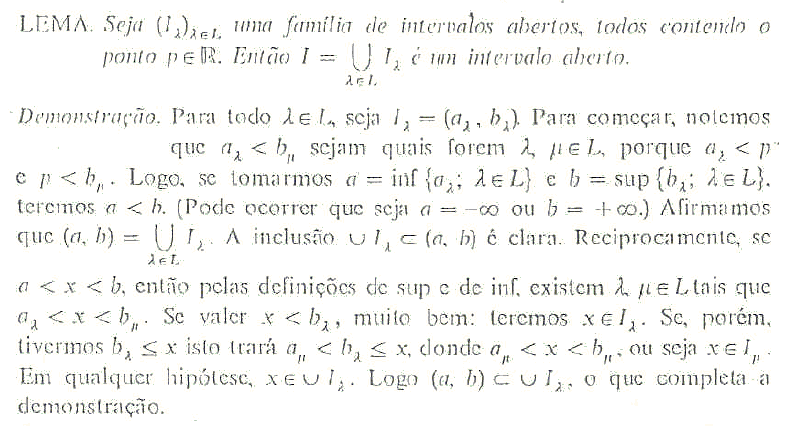
\includegraphics[scale=.9]{lema}
		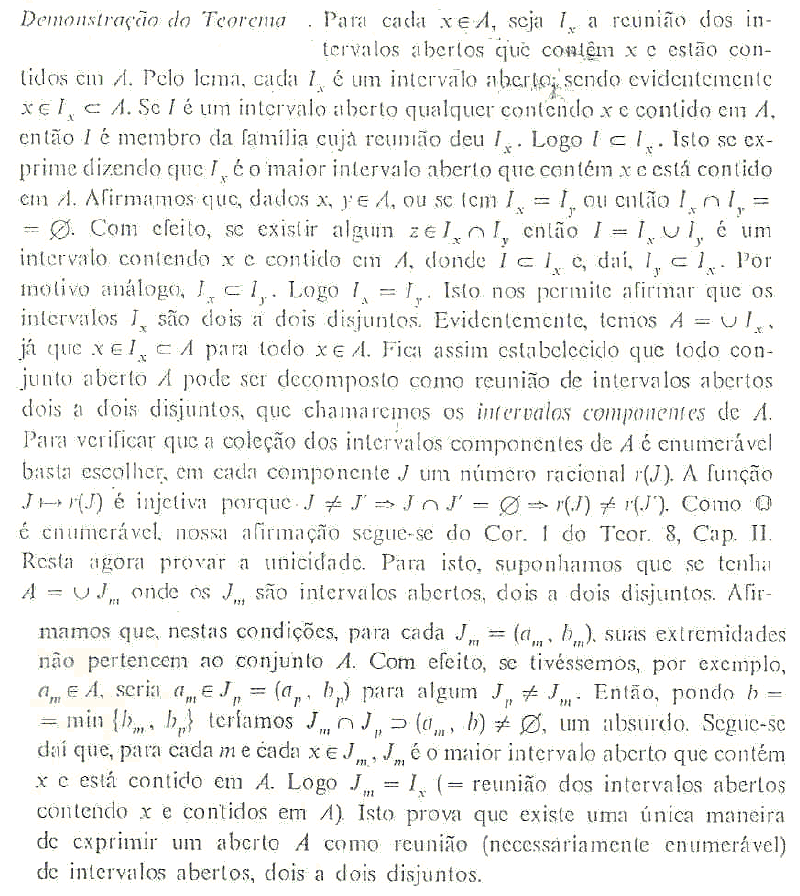
\includegraphics[scale=.9]{teorema}
		\end{center}

\vspace{3mm}

\underline{Corol\'ario $9.1$:} Seja $A \cup B = I$ um intervalo aberto, onde $A, B$ s\~ao conjuntos abertos disjuntos, ent\~ao um desses conjuntos \'e igual a $I$ e o outro \'e igual a $\emptyset$.

Demo: Suponha que $I = A \cup B$ com $A, B$ disjuntos e ambos n\~ao vazios. As decomposi\c{c}\~oes de $A$ e $B$ em seus intervalos componentes d\~ao ao menos $2$ intervalos componentes para $I$. Contradi\c{c}\~ao com a unicidade no lema anterior.

\vspace{100mm}

\underline{Lema $10$:} Sejam $f : X \to \mathbb{R}.\,f \in C^0(a \in X).\,f(a) < k\in \mathbb{R}$ constante. Ent\~ao existe $\delta > 0$ tal que $f(x) < k, \forall x \in X\,;\,|x - a| < \delta$.

Demo: Continuidade $\Rightarrow \forall \epsilon > 0, \exists \delta > 0\,;\,x \in X, | x - a | < \delta \Rightarrow f(a) - \epsilon < f(x) < f(a) + \epsilon$.

Em particular, seja $\epsilon = k - f(a) > 0$. Portanto, $f(x) < k$.

\vspace{3mm}

\underline{Teorema do valor intermedi\'ario:} \textbf{(TVI)} Seja $f : [a, b] \to \mathbb{R}.\,f \in C^0.\,f(a) < d < f(b)$. Ent\~ao existe $c \in (a, b)$ tal que $f(c) = d$.

Demo: $f$ \'e cont\'inua em $a$, ent\~ao para todo $\epsilon = d - f(a) > 0$, existe $\delta > 0$ tal que

$a \le x \le a + \delta \Rightarrow f(x) < f(a) + \epsilon = d$. Todos os pontos $x \in [a, b]$ muito pr\'oximos de $a$ satisfazem $f(x) < d$. $A = \{ x \in (a, b)\,;\,f(x) < d \} \ne \emptyset$.

Analogamente, todos os pontos $y \in [a, b]$ muito pr\'oximos de $b$ satisfazem $d < f(y)$.

$B = \{ y \in (a, b)\,;\,d < f(y) \} \ne \emptyset$.

O lema anterior diz que $A$ e $B$ s\~ao abertos. Suponha por absurdo que n\~ao existe $c \in (a, b)$ tal que $f(c) = d$. Ent\~ao $(a, b) = A \cup B$, em contradi\c{c}\~ao com o corol\'ario $5.1.\,\,\blacksquare$

\underline{Exerc\'icio:} Repita para o caso an\'alogo $f(a) > d > f(b)$.

\vspace{3mm}

O essencial aqui \'e que dada uma curva fechada $\gamma = f(R)$ (suponha que n\~ao se autointercepta: injetiva) inteiramente contida na imagem, cuja pr\'e imagem \'e uma regi\~ao fechada $R$ inteiramente contida no dom\'inio, o teorema garante que todo ponto intermedi\'ario da imagem, possui um (ou mais) pontos na pr\'e-imagem.

\vspace{3mm}

\underline{Lema $11$:} Um subconjunto $X \subset \mathbb{R}$ \'e conexo, se e somente se, \'e um intervalo.

Demo: Sabemos que os intervalos abertos da reta s\~ao conexos. Todo intervalo n\~ao aberto \'e homeomorfo a um destes tr\^es.

$1)\, I = [-1, 1] \Rightarrow f(x) = \sin x$.

$2)\, I = (0, 1] \Rightarrow f(x) = \cfrac{1}{1 + x^2}$.

$3)\, I = [0, \infty) \Rightarrow f(x) = x^2$.

Em todos os casos, $f(\mathbb{R}) = I$ e a imagem de conexo por fun\c{c}\~ao cont\'inua \'e conexa. Reciprocamente, seja $X \subset \mathbb{R}$ um subconjunto conexo. Suponha por absurdo que $X$ n\~ao \'e um intervalo. Ent\~ao existem $a < c < b$ com $a, b \in X; c \notin X$. Setamos $A = (-\infty, c) \cap X\,;\,B = (c, \infty) \cap X$ e obtemos uma cis\~ao $X = A \cup B$, que n\~ao \'e trivial, pois $a \in A, b \in B$. Deixou de ser conexo. Q.E.A.

\vspace{3mm}

\underline{Corol\'ario $11.1$:} A imagem de um conjunto conexo $X \subset \mathbb{R}^n$ por uma fun\c{c}\~ao real cont\'inua $f: X \to \mathbb{R}$ \'e um intervalo.

\vspace{3mm}

\underline{Generaliza\c{c}\~ao $1$:} Seja $f : X \to \mathbb{R}.\,f\in C^0$, definida num conjunto conexo $X \subset \mathbb{R}^n$.

Se existem $\vec a, \vec b\in X\,;\,d\in \mathbb{R}$ tais que $f(\vec a) < d < f(\vec b)$. Ent\~ao existe $\vec c \in X$ tal que $f(\vec c) = d$.

Demo: Simples reformula\c{c}\~ao do corol\'ario anterior.

\vspace{3mm}

\underline{Generaliza\c{c}\~ao $2$:} O dom\'inio \'e qualquer conexo, a imagem \'e qualquer conjunto bem ordenado. Lema de Zorn.

\vspace{12mm}

Fora da caridade, n\~ao h\'a salva\c{c}\~ao. Com caridade, h\'a evolu\c{c}\~ao.

Vinicius Claudino Ferraz, vers\~ao $0.2.0$ de 26/jan/2020.

\end{document}
